\begin{figure}[htbp]
\centering
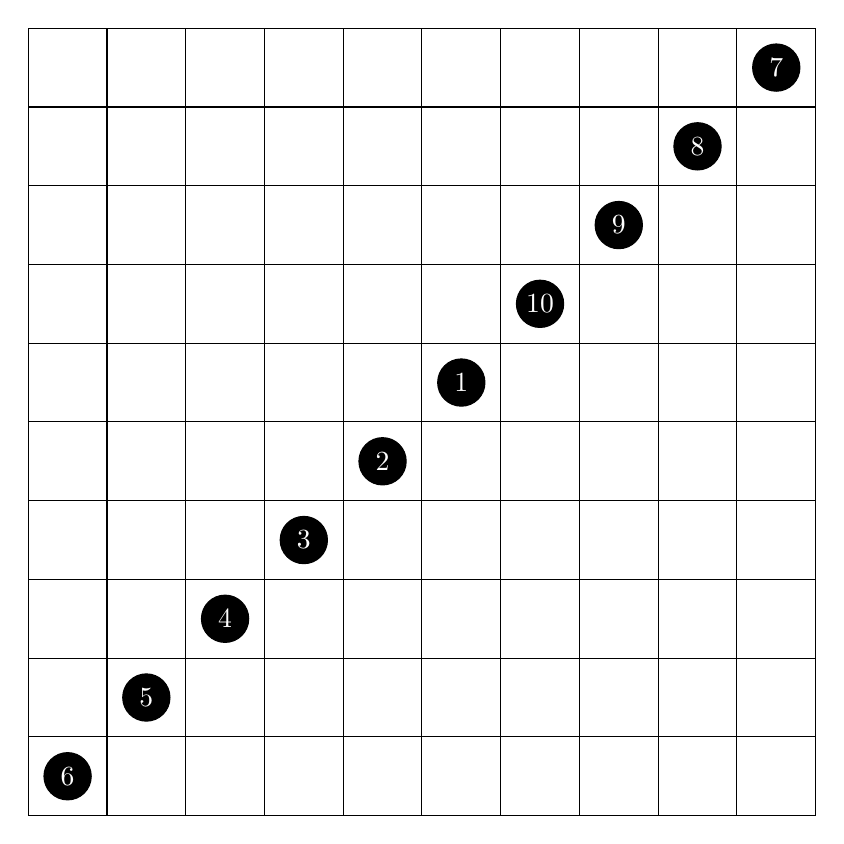
\begin{tikzpicture}

	\draw[xshift=0.5cm, yshift=0.5cm] (0,0) grid (10,10);
	\draw[fill=black] (1, 1) circle [radius=0.3];
	\draw[fill=black] (2, 2) circle [radius=0.3];
	\draw[fill=black] (3, 3) circle [radius=0.3];
	\draw[fill=black] (4, 4)  circle [radius=0.3];
	\draw[fill=black] (5, 5)  circle [radius=0.3];
	\draw[fill=black] (6, 6) circle [radius=0.3];
	\draw[fill=black] (7, 7)  circle [radius=0.3];
	\draw[fill=black] (8, 8)  circle [radius=0.3];
	\draw[fill=black] (9, 9)  circle [radius=0.3];
	\draw[fill=black] (10, 10)  circle [radius=0.3];

	\draw[white] (1, 1) node {6};
	\draw[white] (2, 2) node {5};
	\draw[white] (3, 3) node{4};
	\draw[white] (4, 4) node{3};
	\draw[white] (5, 5) node{2};
	\draw[white] (6, 6) node{1};
	\draw[white] (7, 7) node{10};
	\draw[white] (8, 8) node{9};
	\draw[white] (9, 9) node{8};
	\draw[white] (10, 10) node{7};
	
\end{tikzpicture}

\caption{Soluci\'on del caso de mejor entrada de la Figura \ref{ej_2:mejor}}
\label{ej_2:mejor:sol}
\end{figure}

